% !TeX root = ../main.tex
% Add the above to each chapter to make compiling the PDF easier in some editors.

\section{Memory Usage}
Previously in this thesis for examination of various frame-internal buffers, layers and matrices, Nvidia's Nsight (Visual Studio Edition) allows detailed inspection of almost all runtime information related to a frame's command composition over time and the settings and buffers involved in each command or \textit{event}, as the tool calls it. Nsight was used to read out and briefly discuss the effect of the various optimizations on video memory usage (\autoref{fig:nsight_vmem}). It is, after all, of interest whether any one optimization may easily overflow the VRAM capacity of a particular graphics card. 
For the baseline (all \textit{OFF}) configuration, the following resources are allocated: 

\begin{table}[H]
  \caption[VRAM usage of baseline test configuration}\label{tab:vmem_baseline}
  \centering
  \begin{tabular}{l || S l }
    \toprule
  	\multirow{2}{*}{Resource} & 
  		\multicolumn{2}{c}{memory} \\
        & {footprint (units)} & {type} \\
    \midrule
      Color Buffer	& 137.81MB & (RGBA8 4xSample, 2 layers of 2016x2240) \\
      Depth Buffer	& 139.58MB & (D32, 2 layers of 2016x2240) \\
      Resolve Image	& 17.72MB x2 & (RGBA8 1 layer of 2016x2240) \\
      Asset Textures	& 21.33MB x5 & (RGBA8, 1 layer of 2048x2048) \\
      Env. Textures	& 16.03MB & (RGBA16, 6 layers of 512x512) \\
      Env. Textures	& 528KB & (RGBA32, 6 layers of 64x64) \\
      PBR Reference	& 1024KB & (RG16, 1 layer of 512x512) \\
    \midrule
      Index Buffer	& 1.77MB & (cube + high poly assets geometry) \\
      Instance Model Matrices	& 678.80MB & (64B per instance) \\
    \bottomrule
  \end{tabular}
\end{table} 

Another 257.41MB are used for texture and buffer staging but not used every frame thereafter. A buffer for camera matrices and positions takes up 288B. Additionally 1025 small (about 200-220KB) buffers are used at startup, declared as index buffers, but only about 30 are regularly reused in a frame. For each of the listed buffers, textures and images, a \codeword{DEVICE_LOCAL} memory pool of the corresponding size resides in the GPU onboard memory, model matrices and staging buffers are created as \codeword{HOST_VISIBLE \& HOST_COHERENT} memory to be synchronized between the CPU RAM and GPU VRAM when changed. Such changes may include object transformation via the respective model matrix or upload of new textures to the GPU. \\

Upon activation of any optimizations, only one distinct change is observed. When Stencil Masking is enabled, the depth buffer is created with not only the depth bit set but also the stencil bit and its format is changed from a 32bit SFLOAT to a 32bit SFLOAT along with a layer of 8bit UINT. The effect of this change in resource usage is a size increase of the depth buffer from 139.58MB to a combined depth and stencil buffer with a size of 277.39MB. \\
Apart from this, the other three optimizations have negligible effect on video memory utilization. For each frustum afforded or saved by \gls{MFFR} or the Superfrustum, the camera parameter buffer is expanded or shrunk by 144B. And for each additional frustum the command buffer increases in size, but the change is not easily measurable as the changed frustum sizes and changing draw lists in each frame lead to more fluctuation in the buffer size. \\

The preliminary consensus from these limited measurements is that the implemented optimizations have significant impact only on framebuffer size where the worst - and only different - case means a 49\% footprint increase for Stencil Masking. The total video memory usage change can thus be considered insignificant as scene resources and assets make up the majority of resources. 

\begin{figure}[h!]
  \centering
  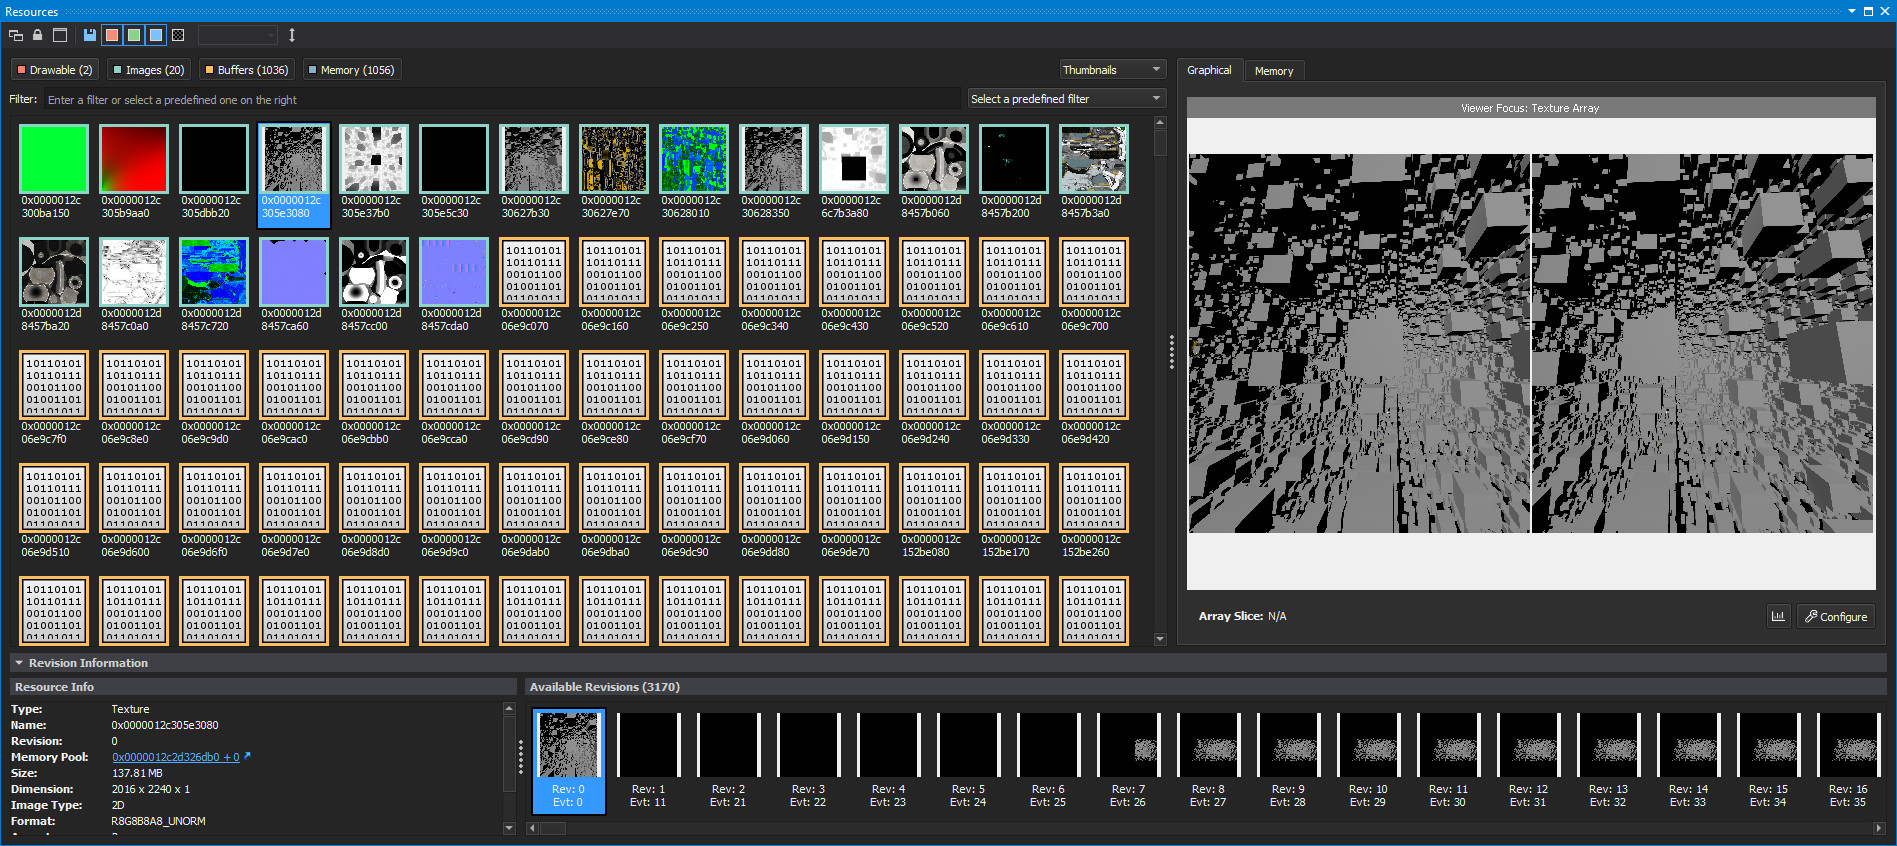
\includegraphics[width=0.9\textwidth]{pictures/nsight_vmem}
  \caption{\textit{Resources} tab of a live Nsight VS frame capture for the baseline test configuration} \label{fig:nsight_vmem}
\end{figure}